
\documentclass{beamer}
\usepackage[utf8]{inputenc}
\usepackage[spanish]{babel}
\usepackage{graphicx}
\usepackage{amsmath, amssymb}
\usepackage{booktabs}
\usepackage{colortbl}
\usepackage{xcolor}
\usepackage{hyperref}

\title{Proyecto Final Diplomatura Universitaria en Ciencia de Datos}
\author{Horacio Antonio Zini}
\date{12 de abril de 2025}

\begin{document}
    \frame{\titlepage}
    \begin{frame}{Introducción}
        A partir de un dataset de ventas mayoristas por cliente y producto, el objetivo del trabajo 
        fue realizar un análisis exploratorio y predictivo del dataset mediante clasificación multiclase 
        entrenando modelos de aprendizaje profundo.
    \end{frame}
    \begin{frame}{Introducci\'on -- Dataset}
        Variables del conjunto de datos: 
        \begin{itemize}
            \item Información sobre el cliente
            \begin{itemize}
                \item User ID: identificación del usuario.
                \item Gender: sexo del usuario.
                \item Age: edad en intervalos.
                \item Ocuppation: ocupación (enmascarada).
                \item Marital Status: estado civil.
                \item City Category: categoría de la ciudad (A,B,C).
                \item Stay In Current City Years: número de años que lleva en la ciudad actual.
            \end{itemize}
            \item Información sobre el producto
                \begin{itemize}
                    \item Product ID: identificación del producto.
                    \item Product Category 1: categoría 1 del producto.
                    \item Product Category 2: categoría 2 del producto.
                    \item Product Category 3: categoría 3 del producto.
                \end{itemize}
            \item Purchase: importe total de la compra del mes pasado.
        \end{itemize}
        La variable objetivo es Purchase.
    \end{frame}
    \begin{frame}{Preprocesamiento -- Análisis exploratorio inicial}
        \begin{table}[ht]
            \centering
            \caption{Tipos de columnas y cantidad de valores únicos.}
            \begin{tabular}{l c c }
                \toprule
                \textbf{Columna} & \textbf{Tipo} & \textbf{Valores únicos} \\
                \midrule
                User ID              & int64   & 5.891  \\
                Product ID           & object  & 3.631  \\
                Gender               & object  & 2      \\
                Age                  & object  & 7      \\
                Occupation           & int64   & 21     \\
                City Category        & object  & 3      \\
                Stay In Current City & object  & 5      \\
                Marital Status       & int64   & 2      \\
                Product Category 1   & int64   & 20     \\
                Product Category 2   & float64 & 17     \\
                Product Category 3   & float64 & 15     \\
                Purchase             & int64   & 18.105 \\
                \bottomrule
            \end{tabular}
            \label{tab:colsdataset}
        \end{table}
    \end{frame}
    \begin{frame}{Preprocesamiento -- Análisis exploratorio inicial}
        Dimensiones del dataset:
        \begin{itemize}
            \item Número de observaciones: 550.068
            \item Número de variables: 12
        \end{itemize}
        Sólo las columnas Product Category 2 y Product Category 3 tienen valores nulos,
        173.638 y 383.247, lo que representa un 32\,\% y un 70\,\%  de valores nulos sobre 
        el total de los datos, respectivamente.
    \end{frame}
    \begin{frame}{Preprocesamiento -- Transformación de variables}
        \begin{table}[ht]
            \centering
            \caption{Codificación de variables categóricas a numéricas.}
            \begin{tabular}{l l l}
                \toprule
                \textbf{Variable} & \textbf{Categoría} & \textbf{Valor codificado} \\
                \midrule
                Gender & F & 0 \\
                    & M & 1 \\
                \midrule
                Age & 0--17 & 0 \\
                    & 18--25 & 1 \\
                    & 26--35 & 2 \\
                    & 36--45 & 3 \\
                    & 46--50 & 4 \\
                    & 51--55 & 5 \\
                    & 55+ & 6 \\
                \midrule
                City Category & \dots \\
                \midrule
                Stay in Current City & \dots \\
                \bottomrule
            \end{tabular}
            \label{tab:codificacion}
        \end{table}
    \end{frame}
    \begin{frame}{Preprocesamiento -- Tratamiento de valores faltantes}
        Para la imputación de valores nulos, en primer lugar se analizó gráficamente la 
        distribución de las columnas Product Category 2 y 
        Product Category 3. Dado que las columnas no tienen una distribución normal, se realizó
        el proceso de imputar los valores nulos respecto a la mediana de cada característica.
    \end{frame}
    \begin{frame}{Modelado predictivo -- División del dataset}
        El conjunto de datos fue dividido en los tres subconjuntos \textit{entrenamiento-validación-pruba} con una 
        proporción de 80-10-10, con el objetivo de entrenar,
        ajustar y evaluar el desempeño del modelo de manera adecuada.
    \end{frame}
    \begin{frame}{Modelado predictivo -- Elección de métrica y baseline model}
        Para evaluar el desempeño de los modelos, se optó por la métrica \textit{F1 score} debido a que 
        proporciona un equilibrio entre la precisión y la recuperación (recall), dos métricas fundamentales 
        en la evaluación de modelos de clasificación multiclase.
        \linebreak\linebreak
        Se optó por aplicar inicialmente un modelo de Regresión Logística como modelo base para establecer un punto
        de comparación con métodos más complejos como los modelos de Deep Learning.
    \end{frame}
    \begin{frame}{Modelado predictivo -- Aprendizaje Profundo}
        Se entrenó el modelo \textit{Multilayer  Perceptron} (MLP) con una arquitectura
        compuesta por cuatro capas lineales \textit{fully connected} con 256, 128 y 64 neuronas respectivamente, cada una seguida por una 
        función de activación $ReLU$, y una capa lineal final sin activación. 
        La red recibe como entrada un vector de dimensión igual al número de variables predictoras y 
        produce una salida correspondiente a la codificación de categorías de la variable objetivo.
        \linebreak
        Para el entrenamiento, se utilizó la función de pérdida \textit{Cross-entropy}, ponderada 
        según la distribución de clases, y el optimizador $SGD$ con una tasa de aprendizaje de 0.01
        y una penalización L2 (parámetro weight decay) de $1e-4$.
        \linebreak
        El modelo fue implementado utilizando PyTorch.
    \end{frame}
    \begin{frame}{Resultados}
        \begin{table}[h]
            \centering
            \caption{Regresión Logística.}
            \begin{tabular}{l c}
                \toprule
                \textbf{Métrica} & \textbf{Valor} \\
                \midrule
                Accuracy   & 0.3889 \\
                Precisión  & 0.3639 \\
                Recall     & 0.3889 \\
                F1-score   & 0.3660 \\
                \bottomrule
            \end{tabular}
            \label{tab:logistica}
        \end{table}
        \begin{table}[h]
            \centering
            \caption{Desempeño del modelo MLP.}
            \begin{tabular}{l c}
                \toprule
                \textbf{Métrica} & \textbf{Valor} \\
                \midrule
                Epoch final             & 39 \\
                Pérdida (Train / Val)   & 0.983 / 0.973 \\
                F1-score (Train / Val)  & 0.500 / 0.491 \\
                \bottomrule
            \end{tabular}
            \label{tab:mlp}
        \end{table}
    \end{frame}
    \begin{frame}{Resultados}
        \begin{figure}[h]
            \centering
            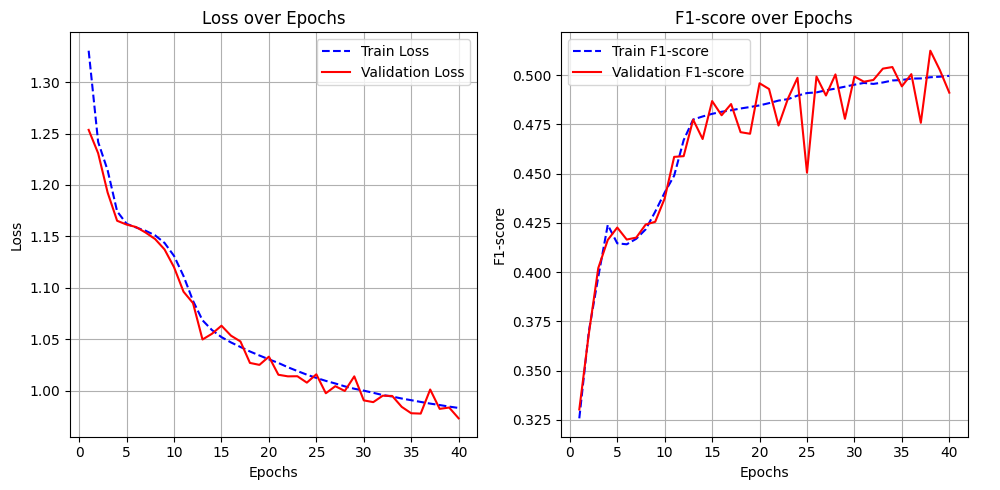
\includegraphics[width=1\textwidth]{loss-f1-epochs.png}
            \caption{Pérdida y Valor-F a lo largo de las épocas}
            \label{fig:mi_imagen}
        \end{figure}
    \end{frame}
    \begin{frame}{Resultados}
        \begin{table}[h!]
            \centering
            \begin{tabular}{c|cccc}
                \rowcolor{gray!30} \textbf{Clase real $\backslash$ Clase predicha} & \textbf{0} & \textbf{1} & \textbf{2} & \textbf{3} \\
                \hline
                \textbf{0} & \cellcolor{yellow!50}10645 & 1346 & 291 & 1473 \\
                \textbf{1} & 6141 & \cellcolor{yellow!50}5601 & 487 & 1530 \\
                \textbf{2} & 3132 & 3727 & \cellcolor{yellow!50}1142 & 5744 \\
                \textbf{3} & 252 & 21 & 364 & \cellcolor{yellow!50}13111 \\
            \end{tabular}
            \caption{Matriz de confusión con colores}
        \end{table}
    \end{frame}
    \begin{frame}{Conclusiones}
        Mientras que el modelo realiza buenas predicciones para las clases extremas, para las clases intermedias 
        se presenta una alta confusión con otras clases. Estas confusiones ocurren principalmente con 
        clases vecinas. Esto sugiere que la representación 
        de los montos medios no está bien diferenciada en el espacio de características. 
        \linebreak
        Teniendo en cuenta que la discretización de la variable continua Purchase se realizó definiendo los 
        límites entre las clases utilizando los cuartiles, las categorías de la variable Purchase y sus rangos quedaron de la siguiente manera:
        \begin{itemize}
            \item Bajo (0): 12 a 5.823
            \item Medio-bajo (1): 5.823 a 8.047
            \item Medio-alto (2): 8.047 a 12.054
            \item Alto (3): 12.054 a 23.961
        \end{itemize}
    \end{frame}
    \begin{frame}{Conclusiones}
        Al observar el tamaño de los intervalos, se nota que las clases intermedias son más pequeñas 
        que las categorías extremas, que abarcan rango mayores. Además, las diferencias entre los 
        valores en las clases 1 y 2 son relativamente pequeños, lo que podría estar dificultando la diferenciación 
        entre ellas durante el entrenamiento del modelo.
        \linebreak
        Esto puede explicar la alta confusión en la clasificación de las clases intermedias, ya que los valores 
        en estos rangos están muy próximos y no presentan una separación clara en el espacio de características del modelo. También 
        explica el buen desempeño del modelo para clasificar elementos de la categoría 3, ya que esta es la clase con el rango más amplio.
    \end{frame}
    \begin{frame}{Conclusiones}
        Es importante notar también que la categorización de la variable objetivo se realizó
        asignando etiquetas numéricas de menor a mayor según el monto de compra.
        \linebreak
        Dado que estos valores representan niveles de compra en una escala lineal sin considerar la diferencia de escala entre los rangos de las clases, 
        el modelo aprende que existe un orden inherente entre las clases pero no necesariamente aprende que la 
        diferencia entre 1 y 2 es menor que la diferencia entre 2 y 3.
        \linebreak
        Esta falta de información sobre las escalas de las clases puede ser una de las razones por las que el 
        modelo tiene dificultades en la distinción de los montos intermedios, y explicaría la confusión observada en la matriz de confusión.
    \end{frame}
\end{document}